\documentclass[a4paper,twoside,11pt]{article}
\usepackage[utf8]{inputenc}
\usepackage[dvipsnames]{xcolor}
\usepackage{amsmath}
\usepackage[a4paper,left=2cm,right=2cm,top=2cm,bottom=2cm]{geometry}
\usepackage{amssymb}
\usepackage{tabularx}
\usepackage{graphicx}
\usepackage[ruled,vlined]{algorithm2e}
\usepackage{listings}
\usepackage{framed} 
\usepackage[english]{babel}
\usepackage{fancyhdr}
\pagestyle{fancy}
\fancyhf{}
\chead{fundamental stat genetics Study Notes}
\lhead{Summer 2021}
\rhead{Caiwei Xiong}
\cfoot{\thepage}
\usepackage[T1]{fontenc}
\usepackage{lmodern}
\usepackage[figurename=Fig.,labelfont=bf,labelsep=period]{caption}
\usepackage{subcaption}
\usepackage{newtxtext,newtxmath}
\definecolor{shadecolor}{rgb}{0.94,0.97,1.0} \definecolor{c1}{HTML}{FFFFCC}


\begin{document}
\tableofcontents
\newpage
\section{Chapter 1 Introduction to Statistical Genetics and Background in Molecular Genetics}
\subsection{Basic Concepts in Genetic Disease}
\textcolor{NavyBlue}{Phenotypes: }The available data for most statistical investigations consisted only of traits. (We use the terms traits and phenotypes here to mean individual characteristics, not observed at the molecular level, which are thought to have a heritable basis.)
\newline
\newline
\textcolor{NavyBlue}{Probands: }Individuals with the disease, called probands, were identified; information on relatives of the probands was used to form family or pedigree structures
\newline
\newline
\textcolor{NavyBlue}{Ascertain: }The term ascertain is used when referring to probands to indicate that the selection of individuals for study may depend on their phenotypes
\newline
\newline
\textcolor{NavyBlue}{\textit{The phenotypes or traits of the relatives and their familial relationships were exploited in a segregation analysis to infer the underlying genetic model.}}
\newline
\newline
\textcolor{NavyBlue}{Genetic markers: }Advances in our understanding of the biology of genetics and in laboratory technology have enabled us to now readily obtain data directly on gene variants, called genetic markers, at specific locations in the genome.
\newline
\newline
\textcolor{NavyBlue}{Gene mapping: }Having marker data for samples of families has enabled gene mapping, which encompasses a variety of methods used to find the chromosomal location of a disease-causing gene.
\newline
\newline
\textcolor{NavyBlue}{Linkage analysis: }
\begin{itemize}
    \item An early statistical approach to gene mapping
    \item Uses marker data and the traits of a pedigree
    \item Very successful in finding genes for Mendelian disorders (i.e., Diseases or disorders which are initiated by variants in a single gene are typically rare and severe conditions)
    \item Less successful with finding genes for complex disorders (i.e., multi-factorial diseases or complex genetic diseases. Here, disease risk is thought to be influenced by a set of genes and environmental factors which may interact with each other.)
\end{itemize}
\textcolor{NavyBlue}{Genome Wide Association Studies (GWAS): }Gene mapping involves scanning the entire human genome at hundreds or thousands or even millions of genetic markers in the genomes of large samples in order to look for genetic variation associated with disease traits
\newline
\newline
\textcolor{NavyBlue}{Genetic Association studies: }A component of gene mapping; their current popularity stems from the advances in genotyping and from information about the structure of genetic variation captured in the HapMap Project. 
\newline
\newline
\textcolor{NavyBlue}{Genetic association analysis: }is distinct from virtually all other types of statistical genetics analyses in that it can be carried out using samples of unrelated individuals rather than families or pedigrees.
\begin{itemize}
    \item using both unrelated samples, and using samples of families
\end{itemize}
\textcolor{NavyBlue}{Population Genetics: }is concerned with the genetic variation within and between populations, over time and space. 
\newline
\newline
Modeling variation in genes due to $\begin{cases}
\text{selection of certain variants due to response to environmental conditions} \\
\text{in- and out-migration} \\
\text{drift occurring in small populations and mutations} \\ 
\text{understanding genetic differences in populations}
\end{cases}$
\newline
\newline
\textcolor{NavyBlue}{Genetic Epidemiology: }is a branch of epidemiology that deals with both genetic and environmental contributions to disease. 
\newline
\newline
\textcolor{Purple}{Two examples of genetic diseases: }
\newline
\begin{itemize}
    \item Sickle Cell Anemia
\newline
This disorder is a common textbook example of a genetic disease because it was the first to be labeled a molecular disorder resulting from a genetic mutation.
    \begin{itemize}
        \item Segregation analyses of African and African-American pedigrees done in the 1920s
        \item 25 years later, segregation analyses using sickle cell disease as the trait correctly identified the genetic nature of sickle cell disorder
        \item About this time, laboratory studies showed that sickling was due to a genetic variant which changed the molecular structure of hemoglobin, enabling scientists to limit their search to the hemoglobin gene without any linkage studies
        \item A decade later, the specific variant in the hemoglobin gene on chromosome 11 was located.
    \end{itemize}
This explains the high prevalence of the variant, and the disorder, in those regions and gives rise to the concept of ‘heterozygote advantage’
    \item Alzheimer’s Disease
\newline
It is a brain disorder with progressive destruction of brain cells leading to loss of memory and other cognitive functions, social impairment and eventually death. 
\end{itemize}
\subsection{Review of Molecular Genetics}
\textcolor{NavyBlue}{Human genome: }The human genome refers to all of the basic biological material that is transmitted from parents to offspring, determining their inherited characteristics.
\newline
\newline
\textcolor{NavyBlue}{Chromosomes: }The heritable material is stored on chromosomes in the nucleus of every cell. There are 23 pairs of chromosomes in the human genome
\newline
\newline
\textcolor{NavyBlue}{Centromere: }The centromere of a chro- mosome is a region found near the middle of the chromosome; it plays an important role in cell division and reproduction.
\newline
\newline
\textcolor{NavyBlue}{DNA: }Each chromosome is composed of long strands of DeoxyriboNucleic Acid (DNA). DNA is the basic biological material of inheritance; it determines how proteins are manufactured in the body.
\begin{itemize}
    \item There are four distinct bases (A, C, T, G) which compose DNA in pairs. The pairing is obligatory: G and C are always paired, and A and T are always paired.
\end{itemize}
\textcolor{NavyBlue}{Genes: }are largely contiguous stretches of DNA that are responsible for making proteins; the beginning and end of a gene are signaled by specific, short DNA sequences. 
\newline
\newline
DNA sequence in a gene consists $\begin{cases} 
\text{coding} \Leftrightarrow \text{exons} \\ (\text{i.e. DNA sequences that make up the exons code for specific proteins determined} \\
\text{by the DNA sequence})
\\
\text{non-coding} \Leftrightarrow \text{introns} \\ \text{(i.e. DNA sequences lying in introns, or sequences lying outside of genes, do not code }\\
\text{for proteins, but are thought to play other important roles in regulating the manufacture} \\
\text{of proteins})
\end{cases}$
\begin{center}
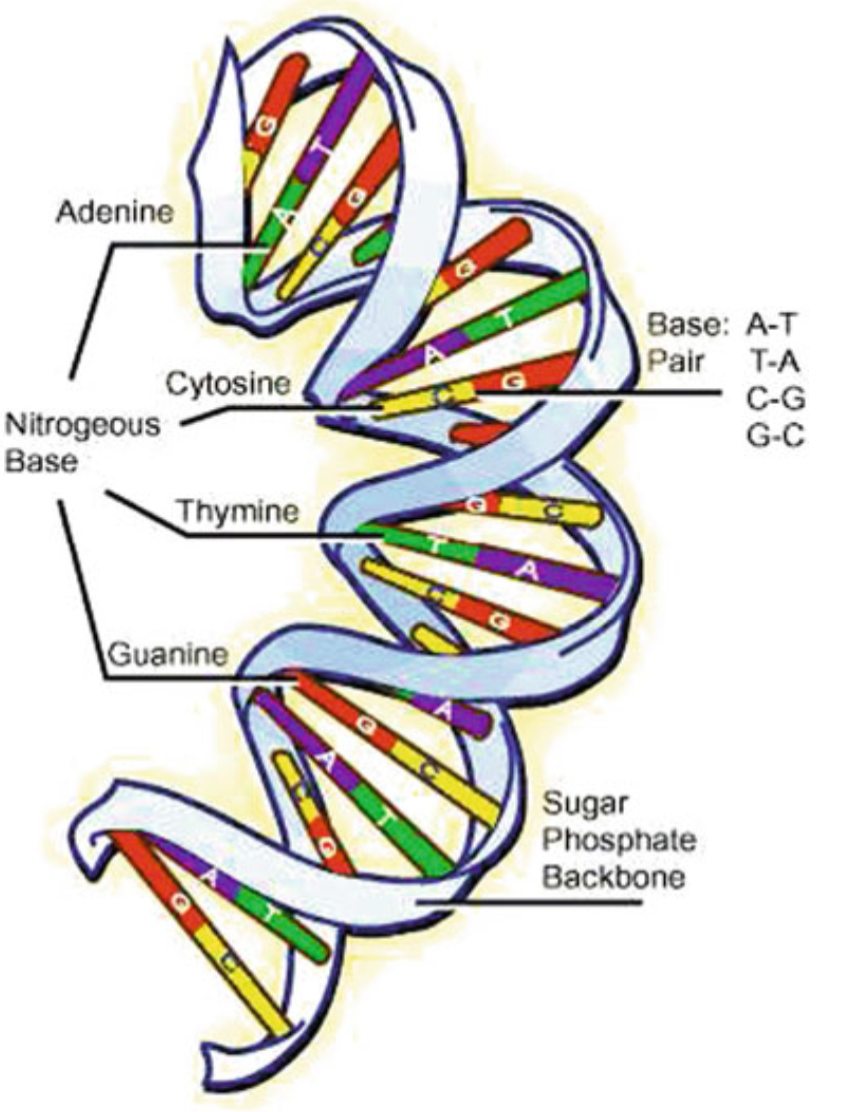
\includegraphics[scale=0.5]{figure1.png}
\end{center}
\begin{itemize}
    \item The focus of gene mapping has historically been to find the location of one or more of the protein coding regions which have variants affecting disease.
    \item Complex disorders may be influenced by genetic variants in non-coding regions as well.
\end{itemize}
\textcolor{NavyBlue}{Genetic locus: }A genetic locus refers to a particular location in a chromosome that is polymorphic.
\newline
\newline
\textcolor{NavyBlue}{Polymorphic: }Polymorphic means that the data at that locus can have more than one possible variant; a polymorphism refers to a polymorphic genetic locus.
\newline
\newline
\textcolor{NavyBlue}{Alleles: }The different variants at a locus are called alleles.
\newline
\newline
\textcolor{NavyBlue}{Polymorphic: }
\begin{itemize}
    \item Historically the minor allele frequency at a locus was required to have population frequency of at least $1\%$ in order for a locus to be considered polymorphic
    \item Recently the term is used loosely to indicate any locus where two or more variants are found, regardless of frequency.
\end{itemize}
\textcolor{NavyBlue}{Homozygous \& Heterozygous: }
\newline
When there are only two possible variants, it is conventional to refer to them as ‘A’ and ‘a’. When dealing with the autosomes
\begin{itemize}
    \item an individual with two copies of A, one on each of the two chromosomes homozygous A, or AA or aa 
    \item an individual with one A and one a is called heterozygous, or Aa 
\end{itemize}
\textcolor{NavyBlue}{Genotype: }The genotype of an individual refers to the pair of alleles at a location, i.e., AA, Aa, or aa. 
\subsection{Types of Genetic Variants}
\textcolor{NavyBlue}{Genetic marker, or just marker: }describe genetic data, observed at the molecular level, at a particular locus that allows us to distinguish genetic differences in individuals.
\newline
\newline
\textcolor{NavyBlue}{Variants: }arise in the coding region of a gene can cause the protein encoded by that gene to malfunction and cells that rely on this protein cannot function properly.
\newline
\newline
\textcolor{NavyBlue}{Genetic disorders or diseases: }Problems for the tissues or organs.Such conditions related to gene mutations, or variants, are called genetic disorders or diseases. Genetic variants which cause a genetic disorder are often referred to as disease mutations.
\newline
\newline
\textcolor{NavyBlue}{Disease susceptibility locus (DSL): }indicates a gene, or specific genetic locus, which has a variant associated with a disease.
\newline
\newline
\textcolor{NavyBlue}{\textit{The term mutation is often used to refer to the event which creates a new variant at the genetic locus and not to the variant itself; we will subsequently adopt that convention here.}}
\newline
\newline
\textcolor{NavyBlue}{Single Nucleotide Polymorphisms (SNP): }The simplest type of genetic marker is a single nucleotide polymorphism (SNP). The double helix structure of DNA requires that each chromosome has complementary base pairs at each location
\begin{center}
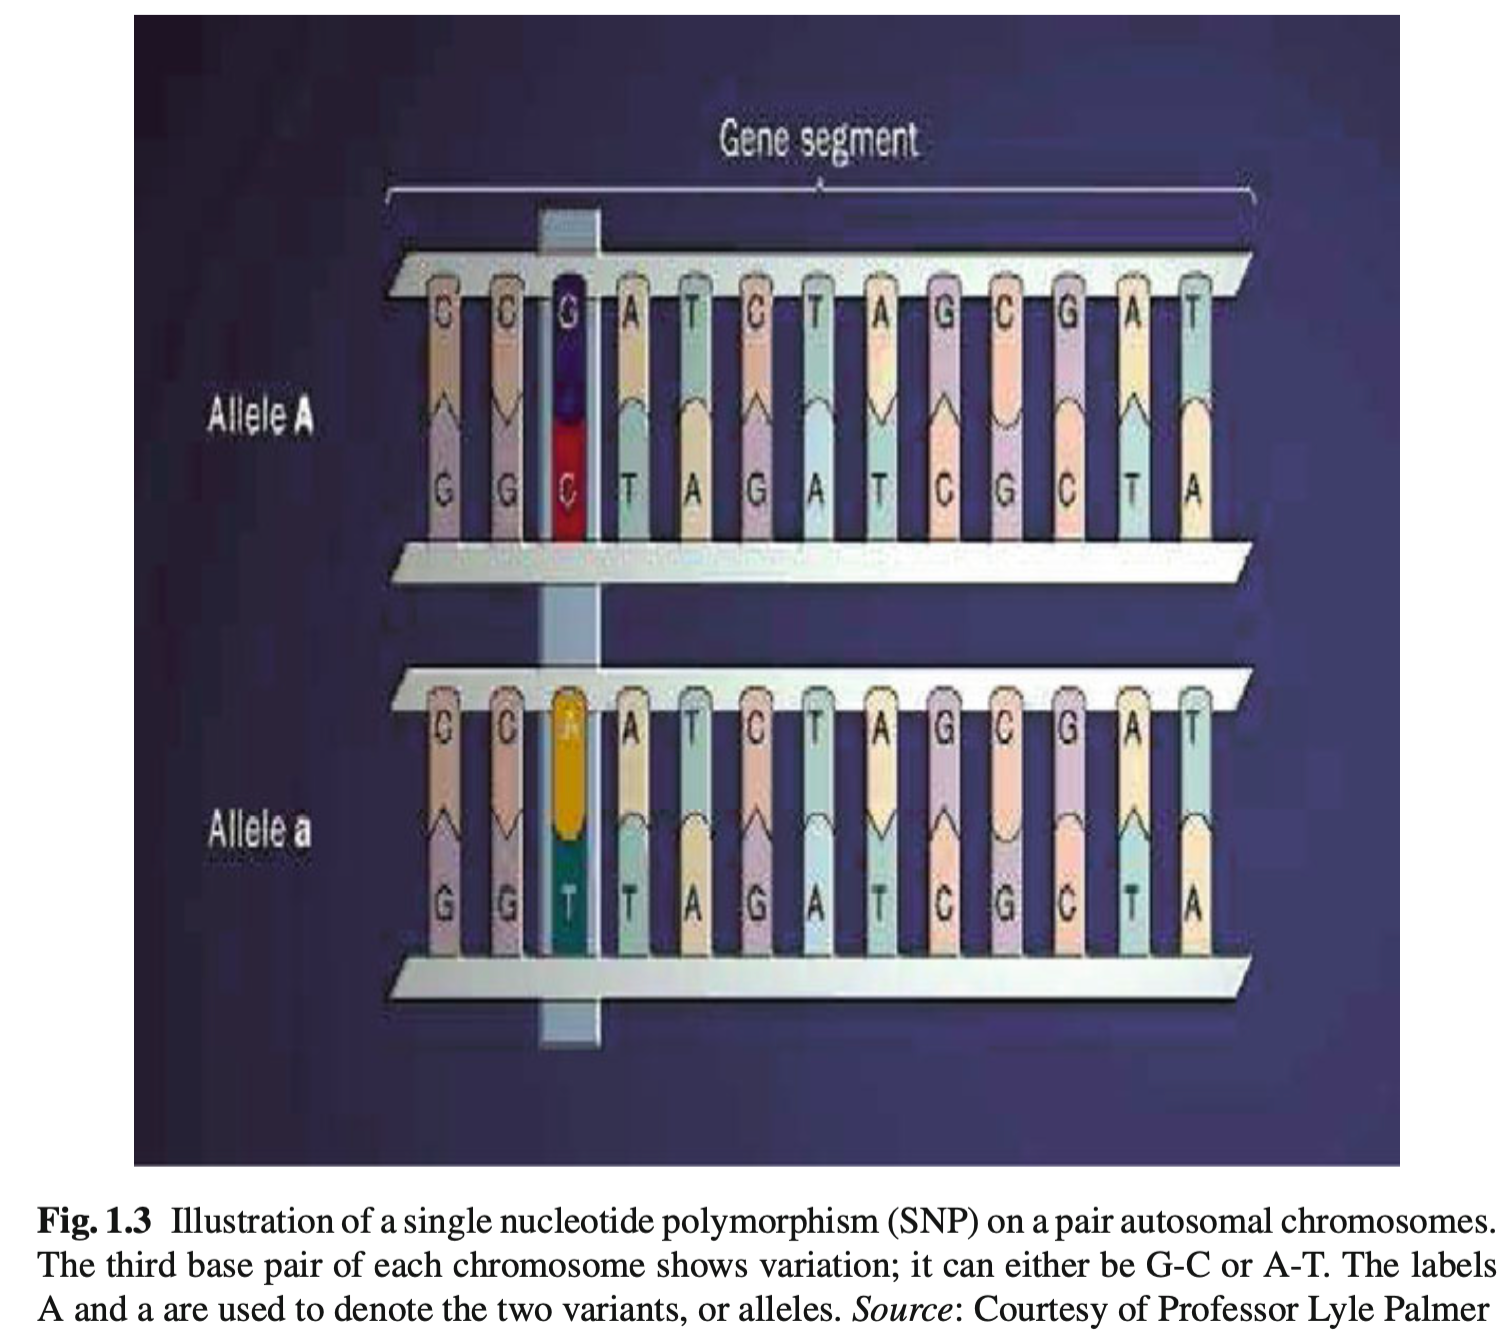
\includegraphics[scale=0.5]{figure2.png}
\end{center}
The two alleles depicted in the figure differ at the third base pair, where an A base is substituted for a G. As we discuss in the next section, whether or not this difference is biologically meaningful depends on where they occur in the DNA sequence and the nature of the letter change.
\newline
\textcolor{NavyBlue}{\textit{SNPs play a very important role in modern gene mapping; they occur commonly throughout the genome and the financial cost of genotyping multiple SNPs at different locations is relatively modest, making them very attractive markers for large scale genetic studies.}}
\newline
\newline
\textcolor{NavyBlue}{Indels: }Extra base pairs (between 1 and 1000 in number) can be inserted or removed (deleted) in between two specific base pairs in a DNA sequence. Collectively, such variants are called indels. They differ from SNPs in that a SNP is merely a substitution and does not change the number of base pairs in the DNA sequence.
\newline
\newline
\textcolor{NavyBlue}{Variable Number of Tandem Repeats (VNTRs): }A common type of variation in DNA consists of specific DNA sequences that are repeated immediately adjacent to each other a variable number of times.
\newline
\newline
\textcolor{NavyBlue}{\textit{The number of repeat base pair sequences can vary widely from one person to the next, microsattelites are excellent markers for distinguishing one person from the next. As such, they are widely used in forensic DNA and paternity testing. They also have been used as the basis of most linkage mapping.}}
\newline
\newline
\textcolor{NavyBlue}{Structural Variants: }Structural variants include many types of chromosomal changes, including rearrangements, duplications, translocations, inversions, deletion or insertions of genetic material.
\begin{center}
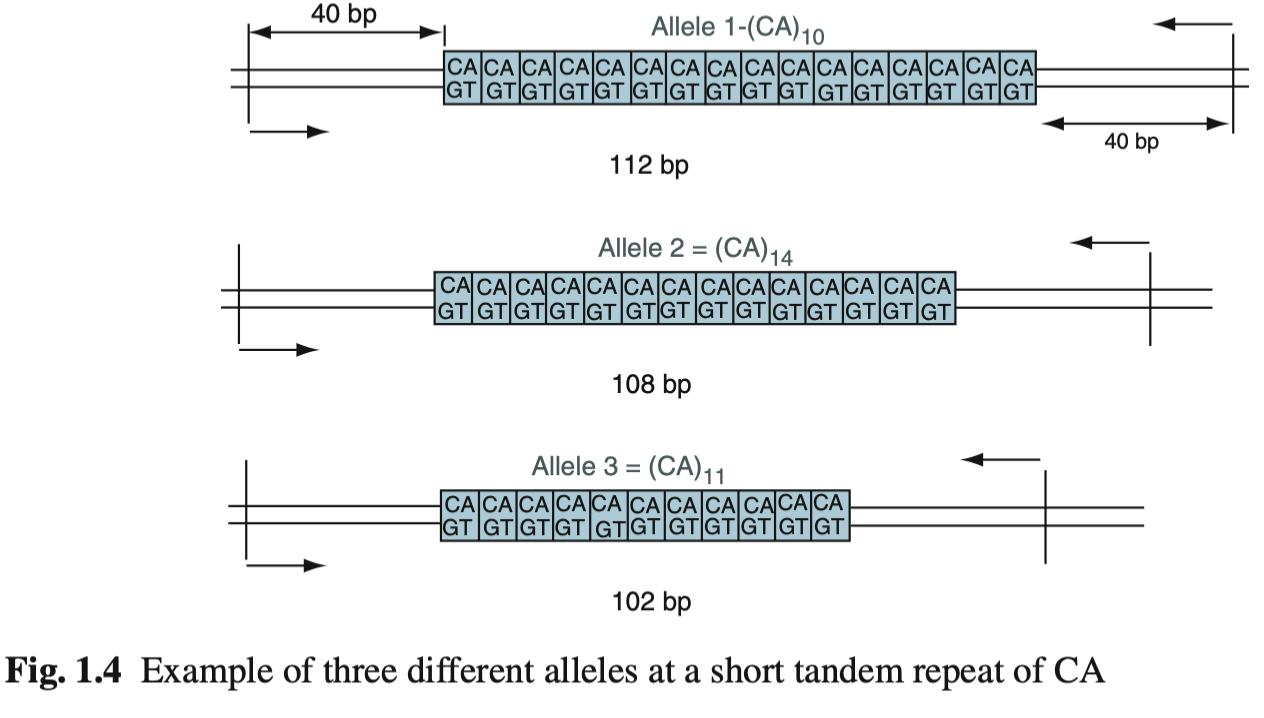
\includegraphics[scale=0.5]{figure3.png}
\end{center}
\subsection{Effects of Genetic Variants on Disease}
SNPs occurring outside a coding region
\begin{itemize}
    \item not to play a role in disease
\end{itemize}
SNPs occurring in a coding region
\begin{itemize}
    \item may not have any biological effects because of some flexibility built into coding sequences
\end{itemize}
\begin{center}
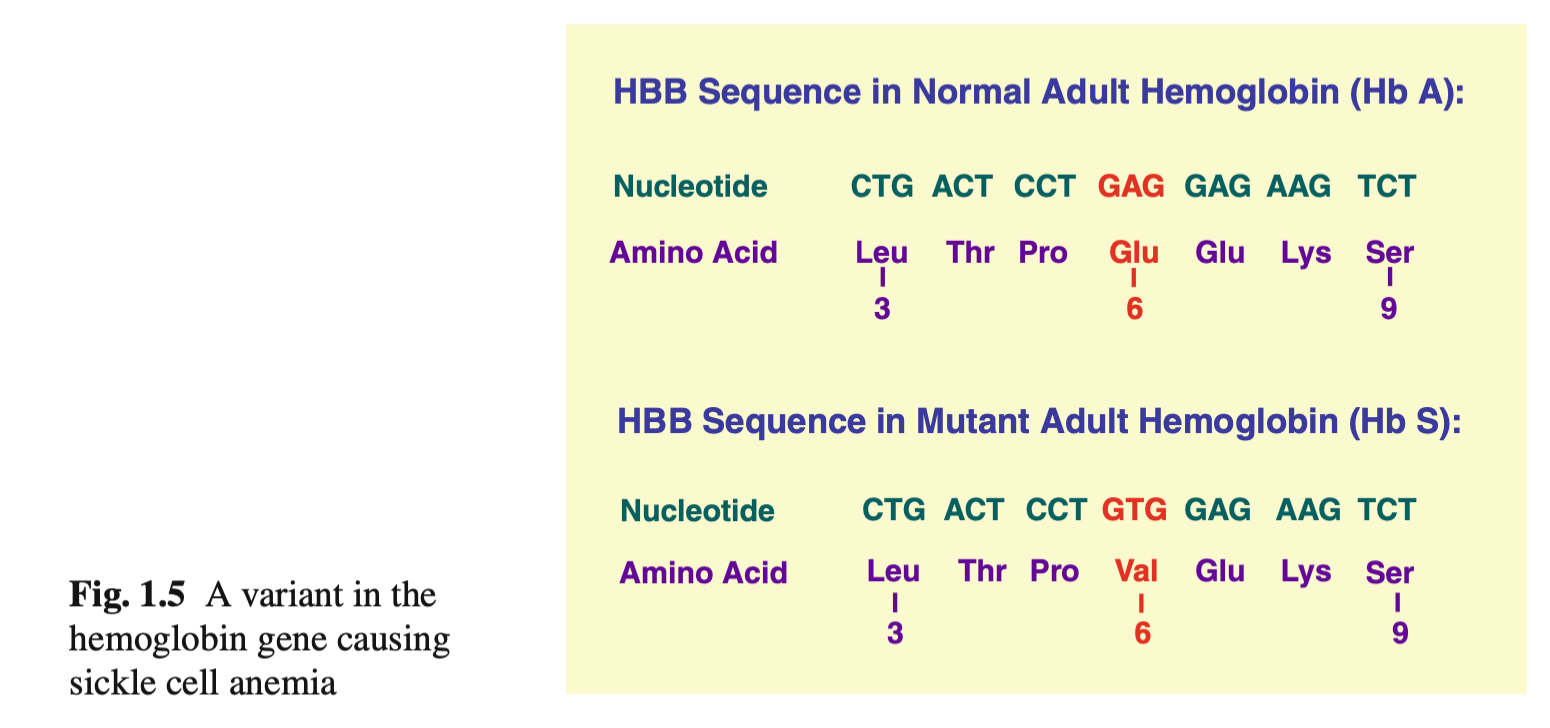
\includegraphics[scale=0.5]{figure4.png}
\end{center}
\textcolor{NavyBlue}{Silent or synonymous: }If the third base in the TCT codon for serine is changed to any one of the other three bases, e.g., TCA, serine will still be encoded. Such variants are said to be silent or synonymous because they cause no change in their product, but they can still be useful as genetic markers.
\section{Chapter 2 Principles of Inheritance: Mendel’s Laws and Genetic Models}
\subsection{Mendel’s Experiments}
Mendel laid out several principles of good experimentation:
\begin{itemize}
    \item using large enough samples of crosses
    \item avoiding unintended cross fertilization
    \item choosing hybrids with no reduction in fertility
\end{itemize}
\textcolor{NavyBlue}{First is the importance of choosing simple, dichotomous traits for study which are easily recognizable and reproducible.} 
\newline
Using dichotomous traits enabled him to use simple genetic models to demonstrate laws of inheritance. It took many decades for scientists to develop models which allowed them to apply Mendel’s laws to continuous traits.
\newline
\newline
\textcolor{NavyBlue}{Second was the use of self-pollinating plants which could also be cross-pollinated; both self-and cross-pollination were used in his experiments.}
\newline
Cross-pollination was used to form the first generation hybrid plants (called F1 in Fig. 2.1); self-pollination was used to develop the parental pure forms (called P in Fig. 2.1), and to infer the genotypes of subsequent crosses. Mendel started the hybridization with the mating of ‘pure’ forms (inbred forms of plants which always yielded the same form of the phenotype, e.g., plants always having either yellow pods or green pods)
\begin{center}
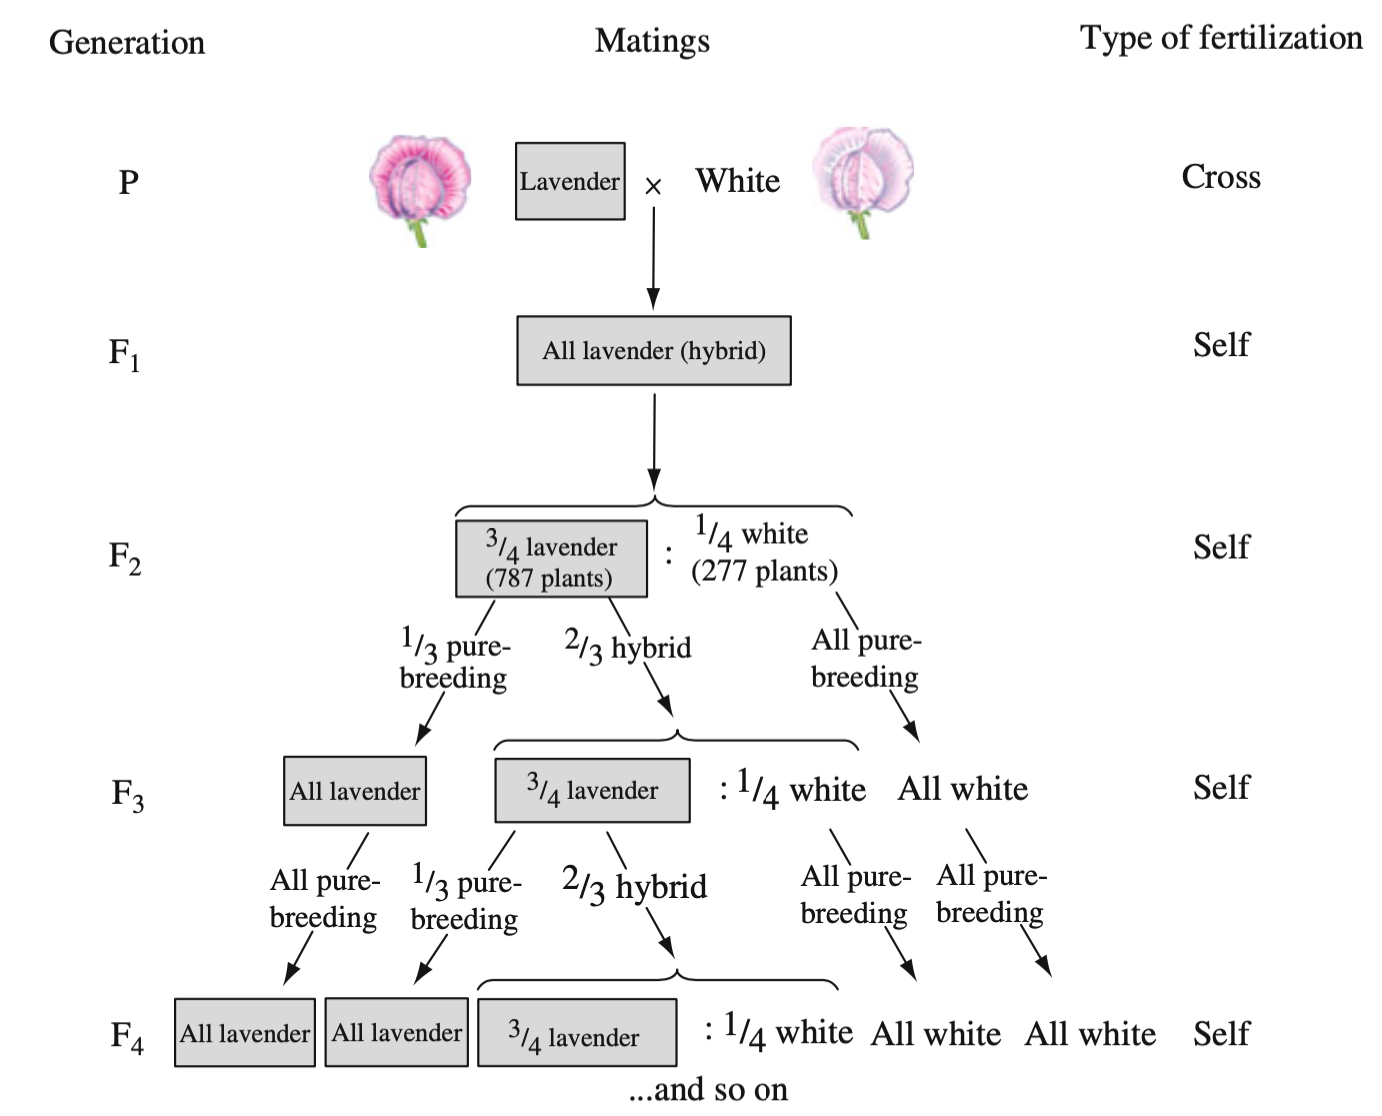
\includegraphics[scale=0.5]{figure5.png}
\end{center}
\begin{itemize}
    \item Mendel started with the simple genetic model for homozygotes:
\end{itemize}
$$
\mathcal{P}(\text{recessive form of trait|aa}) = 1
$$
$$
\mathcal{P}(\text{recessive form of trait|AA}) = 0
$$
$$
\mathcal{P}(\text{dominant form of trait|AA}) = 1
$$
$$
\mathcal{P}(\text{dominant form of trait|aa}) = 0
$$
\textcolor{NavyBlue}{\textit{Note that these models are deterministic; given a genotype, the form of the trait is determined to be either recessive or dominant with probability 1.}}
\begin{itemize}
    \item From the results of the F1 and F2 generations
\end{itemize}
$$
\mathcal{P}(\text{dominant form|Aa}) = 1
$$
$$
\mathcal{P}(\text{recessive form|Aa}) = 0
$$
\begin{itemize}
    \item Subsequent self fertilization over several generations of F2 hybrids
    \begin{itemize}
        \item those plants manifesting the recessive form in the F2 generation produced only recessive forms among their offspring
        \item self fertilization of dominant form could be divided into 2 groups: 
        \begin{itemize}
            \item 1/3 produced only dominant offspring as in pure forms
            \item but 2/3 again produced both recessive and dominant forms in the same ratio seen in the F2 generation of 1:3
        \end{itemize}
    \end{itemize}
\end{itemize}
\begin{shaded*}
\noindent \textbf{Mendel's First Law}
\newline
\noindent Mendel’s First Law (Segregation): One allele of each parent is randomly and independently selected, with probability $\frac{1}{2}$ , for transmission to the offspring; the alleles unite randomly to form the offspring’s genotype.
\end{shaded*}
In summary, the phenotypic ratio for Aa $\times$ Aa matings is $3:1$ (for dominant to recessive forms) and genotypic ratios are $1:2:1$. From Mendel’s law of segregation, one can extend the results to a crossing of arbitrary genotypes, as is shown in Table 2.1. The law of segregation underlies the concept of Mendelian transmissions of alleles from one generation to the next generation
\begin{center}
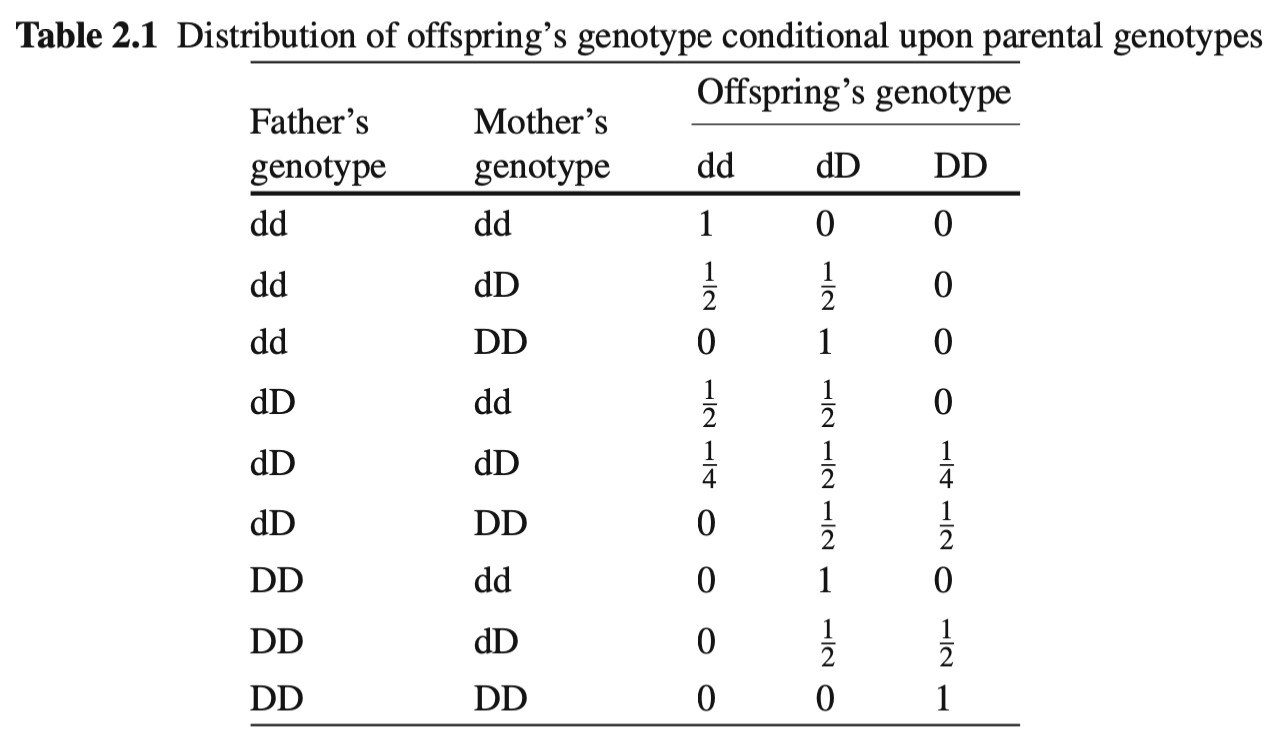
\includegraphics[scale=0.5]{figure6.png}
\end{center}
\begin{shaded*}
\noindent \textbf{Mendel's Second Law}
\newline
\noindent Mendel’s Second Law (Independent Assortment): The alleles underlying two or
more different traits are transmitted to offspring independently of each other; the transmission of each trait separately follows the first law of segregation.
\end{shaded*}
$$
\mathcal{P}(AA \ \text{and} \ BB) = \mathcal{P}(AA) \mathcal{P}(BB) = (1/4)^2
$$
$$
\mathcal{P}(AA \ \text{and} \ Bb) = \mathcal{P}(AA) \mathcal{P}(Bb) = (1/4) \cdot (1/2) = 1/8
$$
\subsection{A Framework for Genetic Models}
\textcolor{NavyBlue}{Genetic Model: }A genetic model describes the relationship, usually probabilistic, between an individual’s genotype and their phenotype or trait.
\newline
We will use the variable $Y$ as the variable that describes the phenotype or trait of interest, whether dichotomous or measured.
\begin{itemize}
    \item $Y=1$ denotes affected
    \item $Y=0$ denotes unaffected
\end{itemize}
\textcolor{NavyBlue}{G: } denote an individual’s genotype
\newline
\newline
\textcolor{NavyBlue}{small-letter a: }Assumed to be the more frequent allele of the two and is referred to as the wild type or normal allele
\newline
\newline
\textcolor{NavyBlue}{capital-letter A: }The less frequent allele is labeled with the capital-letter ‘A’ and referred to as the minor allele (capital letter usually refers to the less common allele.)
\newline
\newline
\textcolor{NavyBlue}{\noindent \textit{Under the assumption that the genetic locus is bi-allelic, each of the two chromosomes has to carry either an ‘a’ or ‘A’ allele, and, consequently, only three different genotypes are possible: the two homozygous genotypes, AA and aa, and the heterozygous genotype Aa. Order does not matter, so Aa is the same as aA. Thus G can take on only three values in a diallelic system. With three alleles, there are 6 possible genotypes, etc. }}
\newline
\newline
If the genetic locus is a \textcolor{NavyBlue}{Disease Susceptibility Locus (DSL)}, it is conventional to use the D/d designation, as opposed to A/a or B/b; the D-allele is then sometimes referred to as the Disease Variant or Disease Susceptibility Allele.
\begin{itemize}
    \item Conditional upon the individual’s genotype G
\end{itemize}
The probabilistic effect of the locus on the phenotype $Y$ is described by the penetrance function which is a set of conditional probabilities, or density functions for continuous phenotypes, which model the distribution of the phenotype/trait $\Rightarrow \mathcal{P}(Y|G)$
\begin{itemize}
    \item If the genetic locus under consideration has no effect on the phenotype of interest
\end{itemize}
The penetrance probabilities for all three genotypes will be equal regardless of the individual’s genotype $\Rightarrow \mathcal{P}(Y|G=dd) = \mathcal{P}(Y|G=dD) = \mathcal{P}(Y|G=DD)$
\newline
\newline
The specification of penetrance probabilities will depend on the type of the disease phenotype. If the phenotype of interest is dichotomous, the penetrance function specifies simple probabilities between zero and one for each genotype, with $\mathcal{P}(Y=1|G) + \mathcal{P}(Y=0|G)=1$ for each $G$
\newline
\newline
\textcolor{NavyBlue}{Y} denotes disease status 
\newline
\textcolor{NavyBlue}{The penetrance probability for $Y=1$} defines the probability of disease conditional on the genotype of the individual
\begin{itemize}
    \item The dominant model holds for the disease outcome
\end{itemize}
$$
\mathcal{P}(Y=1|DD) = \mathcal{P}(Y=1|Dd) = 1 \ \ \text{and} \ \ \mathcal{P}(Y=1|dd)=0
$$
\textcolor{NavyBlue}{D: }denote the disease allele(the variant)
\newline
\textcolor{NavyBlue}{$Y=1$: }refers to the disease 
\begin{itemize}
    \item The recessive model holds for the non-disease outcome
\end{itemize}
$$
\mathcal{P}(Y=1|DD)=1 \ \ \text{and} \ \ \mathcal{P}(Y=1|Dd) = \mathcal{P}(Y=1|dd) = 0
$$
\textcolor{NavyBlue}{\textit{If disease is recessive, it requires two variants, but a dominant disease requires only one. }}
\begin{itemize}
    \item Reduced penetrance 
\newline
If the probability of disease, $\mathcal{P}(Y=1|G)$, is less than $1$ for values of $G$ 
    \begin{itemize}
        \item for the recessive model
$$
\text{for some} \ \ 0 < a < 1 \ \ \ \mathcal{P}(Y=1|DD) = a 
$$
        \item Similarly for the dominant model
    \end{itemize}
    \item Fully penetrant $\Leftrightarrow$ Mendelian models 
\newline
The Mendelian models are called fully penetrant in contrast to reduced penetrance models, because the probability of disease is either zero or one.
\end{itemize}
\begin{center}
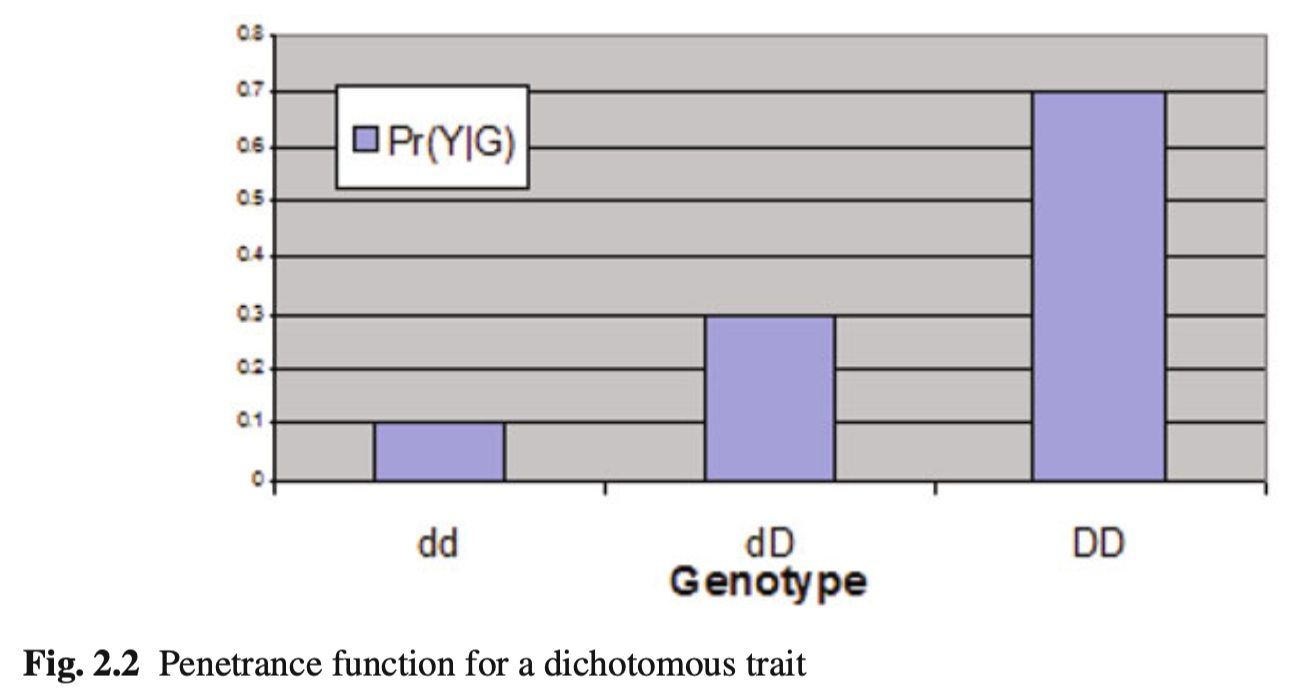
\includegraphics[scale=0.5]{figure7.png}
\end{center}
Probands with the genotype dd have a $10\%$ chance of being affected. For probands with the genotype DD, the probability of being affected is 7 times higher.
\newline
\newline
\textcolor{NavyBlue}{General probability models: }which allow the distribution of Y to depend upon G in some unspecified way.
\newline
\newline
\textcolor{NavyBlue}{Mode of Inheritance: }refers to exactly how parameters of the distribution of Y depend on the number of disease alleles.
\newline
\newline
\textcolor{NavyBlue}{\textit{We generally use the mode of inheritance to indicate how the parameters of the penetrance function depend on the number of disease alleles.}}
\newline
\newline
Four models of inheritance 
\begin{itemize}
    \item recessive
    \item dominant
    \item additive
    \item codominant
\end{itemize}
\textcolor{NavyBlue}{Dominant: }
\begin{itemize}
    \item When only one copy of the disease allele is required to induce an effect on the disease phenotype, $Pr(Y=1|dD)=Pr(Y=1|DD)$
\end{itemize}
Depending on the ‘scale’, with an additive mode of inheritance the penetrance probability of heterozygous genotype is midway between the penetrance probabilities of both homozygous genotypes,
$$
\mathcal{P}(Y=1|Dd) = 0.5 \cdot (\mathcal{P}(Y=1|DD)+ \mathcal{P}(Y=1|dd)) \ \ \text{linear scale}
$$
$$
\mathcal{P}(Y=1|Dd) = \sqrt{\mathcal{P}(Y=1|DD) \cdot \mathcal{P}(Y=1|dd)} \ \ \text{log (multiplicative) scale}
$$
\textcolor{NavyBlue}{Codominant mode of inheritance}
\begin{itemize}
    \item The codominant mode of inheritance makes no assumptions about the relationship among the three penetrance functions, only that they are different.
\end{itemize}
The heterozygote advantage model specifies that heterozygotes have the lowest (or highest for a heterozygote disadvantage model) risk of disease; it is occasionally used, especially in plant breeding.
\begin{shaded*}
\noindent Note: with dichotomous traits, $\mathcal{P}(Y=1|G)$ can be equivalently expressed as $\mathbb{E}(Y|G)$, and likewise for the continuous trait, $\mu_G = \mathbb{E}(Y|G)$
\end{shaded*}
\noindent \textbf{\textcolor{NavyBlue}{Generalized Linear Models (GLM)}}
\newline
\newline
It allows the mean of $Y$ to depend on covariates, $X$, in a non-linear way as:
$$
g(\mathbb{E}(Y|X)) = \beta_0 + X' \beta_1
$$
\begin{itemize}
    \item Logistic link:
$$
\log [\mathbb{E}(Y|X)/(1-\mathbb{E}(Y|X))] = \beta_0 + X' \beta_1
$$
    \item log (relative risk) link:
$$
\log [\mathbb{E}(Y|X)] = \beta_0 + X' \beta_1
$$
\end{itemize}
Here $X$ is a coding of the genotype that reflects the mode of inheritance; it can be a vector or a scalar, depending on the genetic model. 
\newline
\newline
$\beta_1$ gives the additional model parameters which specify how $\mathbb{E}(Y|G)$ depends on G
\begin{center}
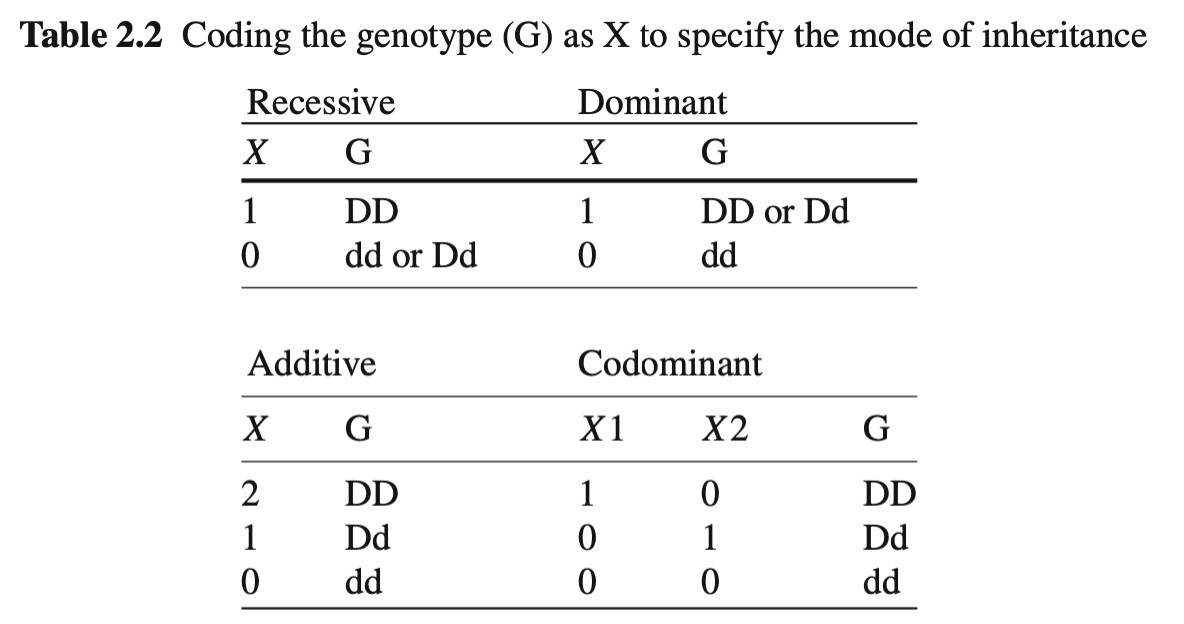
\includegraphics[scale=0.5]{figure8.png}
\end{center}
For the recessive, dominant and additive models:
\newline
\newline
$\beta_1$ is a scalar and defines the ‘effect size’ in the chosen scale; for the codominant model 
\newline
\newline
$\beta_1$ is a vector of length two that gives the effect of the DD and Dd genotypes compared to dd
\subsection{The Biology Underlying Mendelian Inheritance}
\textcolor{NavyBlue}{Diploid: }have two copies of each chromosome (except for males who have one X and one Y for the sex chromosomes). 
\begin{itemize}
    \item One maternal copy
    \item One paternal copy
\end{itemize}
\textcolor{NavyBlue}{Sister chromatids: }Each parental chromosome is first duplicated as illustrated after the first arrow in the top panel. The duplicated chromosomes are called a pair of sister chromatids. 
\newline
\newline
\textcolor{NavyBlue}{Crossover event: }The exchange of material between two non-sister chromatids is called a crossover event
\newline
\newline
\textcolor{NavyBlue}{\textit{Meiosis is not simply randomly choosing one of two parental chromosomes randomly but rather, it allows for creation of additional genetic diversity by mixing of grand parental information within a single chromosome. Each person inherits approximately 1/4 of their genetic material from each of their four grandparents.}}
\newline
\newline
\textcolor{NavyBlue}{\textit{Mendel’s law of independent assortment states that alleles at different genetic loci are transmitted independently from one generation to the next. If they are on different chromosomes, this is naturally the case since each pair of chromosomes undergoes the process of meiosis independently. This creates a substantial amount of genetic variation, even without crossing-over; with crossing-over, the possible combinations are essentially infinite.}}
\begin{center}
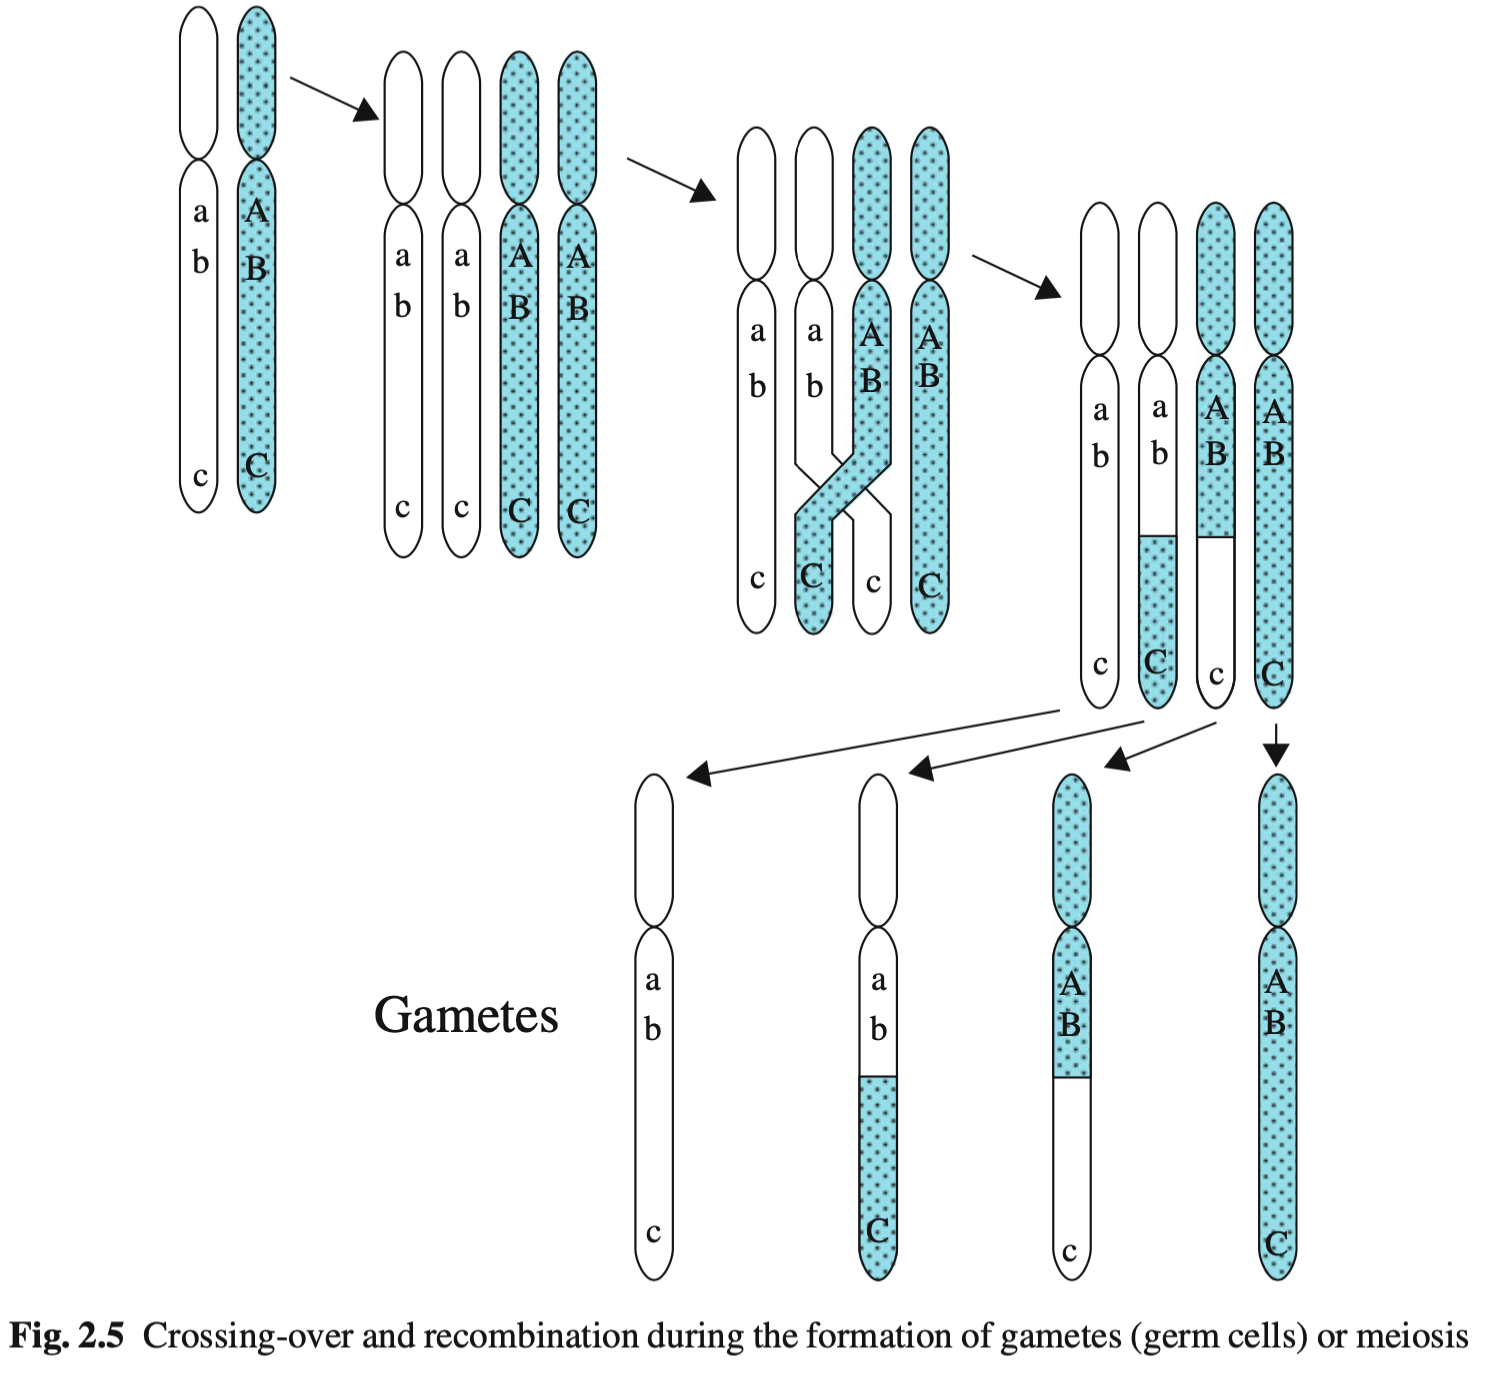
\includegraphics[scale=0.5]{figure9.png}
\end{center}
\textcolor{NavyBlue}{Crossovers:} 
\begin{itemize}
    \item random events in the sense that they cannot be predicted with certainty
    \item they do not occur uniformly or independently along the chromosome
    \item crossover rates can vary by sex, chromosomal region as well as chromosome number, individual and temperature
    \item relatively rare at the centromere and at the ends of a chromosome. 
    \item inherently unobservable
\end{itemize}
\section{Chapter 3 Some Basic Concepts from Population Genetics}
\subsection{Estimation of Allele Frequencies}
\begin{itemize}
    \item Consider estimation of the population proportion of a particular allele, $A$, at a locus
    \begin{itemize}
        \item all other alleles be denoted by ‘$a$’
    \end{itemize}
    \item The allele proportion in the population is defined as the proportion of chromosomes carrying that allele, regardless of the pairing within individuals.
    \item Suppose we have a sample of size $n$ from a population with proportion $p$ of $A$ alleles
    \item Estimate $p$
    \begin{itemize}
        \item Count the number of chromosomes carrying the $A$ alleles and divide by $2n$(the number of chromosomes)
    \end{itemize}
\end{itemize}
\begin{shaded*}
\noindent \textbf{Box 3.1 Calculation of Estimated Allele Frequencies from a Sample of n Subjects}
\newline
\newline
Genotype counts from the sample:
\newline
\newline
$n_{AA} = $ number out of $n$ with genotype $AA$
\newline
$n_{Aa} = $ number out of $n$ with genotype $Aa$
\newline
$n_{aa} = $ number out of $n$ with genotype $aa$
\newline
\newline
where $n_{AA} + n_{Aa} + n_{aa} = n$. The sample proportion of $A$ alleles
$$
\bar{p} = (2n_{AA} + n_{Aa}) /2n
$$
estimates the population proportion of $A$ alleles. With a two allele system, the proportion of a alleles is $\bar{q} = 1- \bar{p}$, as can be verified by exchanging a with A in formula previous
\end{shaded*}
\textcolor{NavyBlue}{\textit{A comment on notation: It is typical in genetics to refer to $\bar{p}$ as the ‘$A$ allele frequency’, even though it is a proportion, and frequency usually refers to a count.}}
\newline
\newline
$\bar{p} \Leftrightarrow$ ordinary proportion \ \ \ \ \ \ \ \ \ $2n \Leftrightarrow$ sample size (the number of chromosomes)
\newline
It is easily seen to be unbiased for the population frequency $p$ provided we have a random sample with equal probability sampling, even if the sample contains relatives.
\newline
\newline
Equal probability sampling: 
\begin{itemize}
    \item requires that everyone in the population has the same probability of being included in the sample.
    \item In practice
    \begin{itemize}
        \item what we need is that the probability of selection into the sample does not depend upon an individual’s genotype or any phenotype related to the genotype. 
    \end{itemize}
\end{itemize}
\textcolor{Purple}{For example to estimate the $3$ allele frequencies at the $ABO$ blood group locus, we must genotype sample individuals without regard to their blood group membership ($A$, $B$, $AB$ or $O$).}
\newline
\newline
\textbf{The usual standard error for a proportion may not hold}: $\sqrt{\bar{p}(1-\bar{p})}/2n$ (because of independence of the $2n$ sampled chromosomes. 
\newline
\newline
Extension to more than $2$ alleles, say $A$, $B$, $C$, etc. is straightforward:
$$
\bar{P}_A = (2n_{AA} + n_{AB} + n_{AC} + \cdots )/2n
$$
Estimation of allele frequencies for the MN blood group is illustrated:
\begin{shaded*}
\noindent \textbf{Box 3.2 Example – estimating allele frequencies for the MN Blood Group}
\newline
\newline
An individual’s $MN$ blood group is determined by a gene with two alleles, $M$ and $N$; they control the amount of $M$ and $N$ antigens on the surface of blood cells. The data below come from two different samples of Eskimos in Greenland. We use the data to estimate the $M$ allele frequency.
\begin{center}
\centering
\begin{tabularx}{1.0\textwidth} { 
  | >{\centeringt\arraybackslash}X 
  | >{\centering\arraybackslash}X
  | >{\centering\arraybackslash}X
  | >{\centering\arraybackslash}X 
  | >{\centering\arraybackslash}X
  | >{\centering\arraybackslash}X 
  | >{\centering\arraybackslash}X | }
\hline
 Location & $MM$ & $MN$ & $NN$ & Total & $\bar{p}$ & $\bar{q}$ \\
\hline
 South West Greenland & $126$ & $53$ & $8$ & $187$ & $0.8155$ & $0.1845$ \\
\hline
 East Greenland & $475$ & $89$ & $5$ & $569$ & $0.9130$ & $0.0870$ \\
\hline
\end{tabularx}
\end{center}
For South West Greenland:
$$
\bar{p} = (2 \cdot 126 + 53)/(2 \cdot 187) = 0.8165
$$
$$
\bar{q} = (2 \cdot 8 + 53)/(2 \cdot 187) = 0.1835 = 1- 0.8165
$$
East Greenland:
$$
\bar{p} = (2 \cdot 475 + 89)/(2 \cdot 569) = 0.9135
$$
$$
\bar{q} = (2 \cdot 5 + 89)/(2 \cdot 569) = 0.0870
$$
\end{shaded*}
\noindent Allele Counting is sometimes used to refer to formula, and also more generally to a method of estimating allele frequencies when data on genotypes are not available directly, but data are available on Mendelian phenotypes, such as $ABO$ blood types.

\subsection{Population Substructure}
\textcolor{NavyBlue}{Population substructure loosely: }Refer to features of a population which result in variation of expected allele frequencies across individuals in a population.

\subsubsection{Population Stratification}
\textcolor{NavyBlue}{Population stratification}: is perhaps the simplest form of population substructure
\begin{itemize}
    \item coincides with the intuitive notion that individuals in a population can be subdivided into mutually exclusive strata
    \item within each strata the allele frequency is the same for all individuals
    \item but it varies between strata
\end{itemize}
Typically we assume that the different strata represent different racial, ethnic and/or geographic subgroups.
\subsubsection{Population Admixture}
\textcolor{NavyBlue}{Population admixture: }refers to a situation where individuals in a population have a mixture of different genetic ancestries due to the mixing of two or more populations at a previous point in time.
\newline
\newline
\textcolor{NavyBlue}{\textit{Most admixed populations are the result of a migration of one or more population groups from specific regions into a different geographic location with a previously settled population.}}
\newline
If the allele frequencies differ in the original ancestral populations
\begin{itemize}
    \item the probability that an individual has a particular allele depends upon the mixture of that individual’s ancestry
\end{itemize}
Population admixture is a more realistic model for most modern population groups than is stratification. 
\newline
\newline
\textcolor{NavyBlue}{Ancestry Informative Marker (AIM)}: a marker with strong differences among population subtypes
\subsubsection{Population Inbreeding}
\textcolor{NavyBlue}{Population inbreeding: }occurs when there is a preference for mating among relatives in a population or because geographic isolation of subgroups restricts mating choices.
\begin{itemize}
    \item there is the possibility that an offspring will inherit two copies of the same ancestral allele
\end{itemize}
\textcolor{NavyBlue}{Inbreeding coefficient: }denoted by $F$, is the probability that a random individual in the population inherits two copies of the same allele from a common ancestor.
\begin{itemize}
    \item In large, randomly mating populations the chances that any two mating parents have a common ancestor allele is low, hence $F$ is negligible and often considered to be zero
    \item Inbred populations have non-negligible inbreeding coefficients
    \begin{itemize}
        \item At the extreme, self-breeding populations of plants have inbreeding coefficients of one
        \begin{enumerate}
            \item All offspring from this self-fertilizing plant have a probability of $1/2$ of inheriting two copies of the same allele
            \item In the next generation, this probability increases to $3/4$, and eventually one of the allele frequencies goes to $1$ in these plants.
        \end{enumerate}
    \end{itemize}
\end{itemize}
In real populations, it is difficult to estimate F exactly, as other phenomena may mimic the effect of inbreeding. Inbred populations have higher than expected frequencies of rare recessive disorders, because inbreeding tends to increase the number of homozygotes in the population.
\subsection{Hardy-Weinberg Equilibrium}
There are many assumptions required for the formula to hold: random mating, no inbreeding, infinite population size, discrete generations, equal allele frequencies in males and females, and no mutation, migration, or selection (meaning that certain alleles do not confer a selective advantage or disadvantage in reproduction).
\newline
\newline
\textcolor{NavyBlue}{$p$: }be the frequency of the A allele in a population satisfying the assumptions given above
$$
\begin{cases}
P(AA \ \text{genotype} ) = p^2 \\
P(Aa \ \text{genotype} ) = 2pq \\
P(aa \ \text{genotype} ) = q%2
\end{cases}
$$
A population is said to be in Hardy-Weinberg Equilibrium (HWE) if the genotypes in the entire population satisfy the equation. Since $(2p^2 + 2pq)/2 = p$, the frequency of $A$ allele among the offspring chromosomes is also $p$. Thus, with HWE, allele frequencies will not change from generation to generation.
\newline
\newline
\textcolor{NavyBlue}{Random mating: }
\begin{itemize}
    \item  the probabilities of the number of $A$ alleles in the offspring generation are given by the binomial formula with probability equal to the A allele frequency and the number of trials equal to $2$
    \item number of $A$ alleles in an offspring is distributed as $B(2,p)$
    \item  the number of $A$ alleles in a random sample of size $n$ from the population is $B(2n,p)$
    \item The formula for $Var(\bar{p})$ from a sample size $n$ is given by the simple binomial formula $\bar{p}\bar{q}/(2n)$
\end{itemize}
\begin{shaded*}
\noindent \textbf{Box 3.3 Inference About allele frequencies in a sample from a population in Hardy-Weinberg equilibrium}
\newline
\newline
Let $i$ index the individuals in a random sample of n independent individuals from a population with allele frequency $p$; let $X_i(i=1,\cdots n)$ denote the number of $A$ alleles for the $i^{\text{th}}$ person in the sample and let $X_+$ denote the summation of $X_i$ over all $n$ individuals. Then we may rewrite $\bar{p}$ as
$$
\bar{p} = \sum^n_{i=1} X_i/2n = X_+ /2n
$$
Since each $X_i$ is distributed as $B(2,p), \mathbb{E}(X_i) = 2p \ Var(X_i) = 2pq$ and with a sample of independent individuals, $X_+$ is $B(2n,p)$ it follows that:
$$
\mathbb{E}(\bar{p}) = \mathbb{E}(X_+)/2n = p
$$
and
$$
Var(\bar{p}) = Var(X_+) /(2n)^2 = pq/2n
$$
In large samples, $\bar{p}$ is approximately $N(p, \bar{p}\bar{q}/2n)$; large sample tests and confidence intervals use this normal approximation. In particular, with large samples, to test $H_0: p=p_0$ at the $\alpha$-level, we reject if the magnitude of
$$
Z = \sqrt{2n}(\bar{p}-p_0)/\sqrt{p_0(1-p_0)}
$$
is greater than the $(1-\alpha)/2$ - percentile $(Z_{(1-\alpha)/2})$ of a standard normal distribution. An approximate $100(1-\alpha)\%$ confidence interval for the true frequency is given by
$$
\bar{p} \pm (Z_{(1-\alpha)/2}) \sqrt{\bar{p}(1-\bar{p})/2n}
$$
The approximations are reasonably good for $n\bar{p} \ge 5$ and $n(1-\bar{p})  \ge 5$ for levels of $\alpha$ close to $0.05$. With smaller samples and smaller levels of $\alpha$, exact inference for $p$ is based on the fact that $X_+$ is $B(2n, p)$.
\end{shaded*}
Note that there is no assumption made about the genotype distribution in the parental population, only that the allele frequency is $p$.
\newline
\newline
\textcolor{NavyBlue}{\textit{The parental population need not follow HWE, that is, the genotypes in the parental population do not follow equation}}
\newline
\newline
However, HWE can be achieved in the offspring in only one generation of random mating, provided the other conditions hold. HWE can also be proved by explicitly considering an arbitrary genotype distribution in the parents, still with allele frequency $p$, and showing that formula holds for the offspring distribution.
\subsubsection{Testing for HWE}

\begin{shaded*}
\noindent \textbf{Box 3.4 The Pearson goodness of fit test for HWE}
\newline
\newline
$H_0:$ HWE holds in the population.
\newline
$H_A:$ HWE does not hold.
\newline
\newline
Given a sample of size n from the population:
\begin{center}
\centering
\begin{tabularx}{1.0\textwidth} { 
  | >{\centeringt\arraybackslash}X 
   >{\centering\arraybackslash}X
   >{\centering\arraybackslash}X
   >{\centering\arraybackslash}X 
   >{\centering\arraybackslash}X
  | >{\centering\arraybackslash}X 
  | >{\centering\arraybackslash}X | }
\hline
 \ & Genotype & \ & \ & \ \\

 \ & $AA$ & $Aa$ & $ aa$ & \ \\
\hline
Observed & $n_{AA}$ & $n_{Aa}$ & $n_{aa}$ & $n$ \\
Expected & $n \bar{p}^2$ & $2n \widebar{pq}$ & $n \bar{q}^2$ & $n$ \\
\hline
\end{tabularx}
\end{center}
$\bar{p}=(2n_{AA} + n_{Aa}/(2n)$
\newline
GOF $\chi^2 = \sum (O-E)^2/E$ is distributed as $\chi^2$ with one degree of freedom under $H_0$, where summation is overall all $3$ genotypes.
\end{shaded*}
\textcolor{Purple}{Example: CCR-5 Deletion} 
\newline
\newline
$CCR-5$ is a chemokind receptor which is involved in the human immune system. It enables the HIV virus to infect the $CD4(+)$ T cells in ‘normal’ individuals and is necessary for AIDS to develop. A deletion of 32 base pairs causes the coding of incorrect amino acids, leading to a disruption of the normal functioning of the receptors. Because the mutation protects against HIV, we might expect to see an excess of two deletions in a sample of AIDS-free individuals.
\newline
\newline
\textcolor{NavyBlue}{\textit{The chi-square test is not significant but the sample is small, especially the number of rare homozygotes; the pattern of observed genotypes is consistent with the idea that AIDS free individuals show an excess of two deletions.}}
\newline
\newline
Pearson’s chi-square test is a \textcolor{NavyBlue}{large sample test}, and the usual recommendation for its validity is that the expected value in each cell is greater than $5$.
\newline
\newline
An exact test which is valid for \textcolor{NavyBlue}{small samples} is based on the idea that the number of heterozygotes will be either too big or too small if HWE fails.
\begin{itemize}
    \item We can compute an exact test of HWE based on the number of observed heterozygotes, conditioning on the number of minor alleles that are observed (or on $\bar{p}$) and using the resulting hypergeometric distribution.
\end{itemize}
\subsubsection{Some Causes of the Failure of HWE}
Rejecting a test of HWE provides some evidence that HWE does not hold in the population. 
\begin{itemize}
    \item population substructure
    \item selection 
    \item genotyping errors
\end{itemize}
In general, the rejection of the test does not indicate a reason for failure, but there are some predictable patterns. 
\newline
\newline
\textcolor{NavyBlue}{\textit{Exactly what happens to the genotype probabilities and/or $Var(\bar{p})$ depends on many features of the population, but the method of sampling and/or genotyping can also affect whether or not HWE will hold in the sample.}}
\newline
\newline
Let $X$ be defined as the number of $A$ alleles, except we drop the $i$ subscript for simplicity. By definition:
$$
\mathcal{P}(X=0) = \mathcal{P}_{aa}
$$
$$
\mathcal{P}(X=1) = \mathcal{P}_{Aa}
$$
$$
\mathcal{P}(X=2) = \mathcal{P}_{AA}
$$
It follows by definition that:
$$
\mathbb{E}(X) = 2 p_{AA} + p_{Aa} = 2p
$$
and
$$
Var(X) = 4p_{AA} + p_{Aa} - 4p^2
$$

\subsubsection{Measuring the Departure from HWE}
















































\end{document}
